\renewcommand\evenpagerightmark{{\scshape\small Diagnostic}}
\chapter[DiagnosticMeasurement]%
{DiagnosticMeasurement}
\label{diagnostic_chapt}

\section{Strioscopy}

\subsection{Opportunities}

What we would like to measure :

\begin{itemize}
\item velocity field
\item density field
\item turbulence field
\item mixture field
\item recirculation zone
\end{itemize}

What we are sure we can measure if the experiments works perfectly  :

\begin{itemize}
\item qualitative representation of the mixture
\item qualitative idea of the turbulence 
\item recirculation zone
\end{itemize}



\subsection{According to the user guide}

Possible to compute quantitatively the density, the temperature (assuming that we know the pressure), even some velocity values... It is very well described, the calculations are very long and not automatized in a script (feasibility?)

\section{Procedure}

\subsection{What is needed}

\begin{itemize}
\item The strioscopy
\item a dilution facility 
\item A thermocouple
\item A calibrated movable pedestal
\item A CCD camera (when the whole diagnostic is proven to work)
\item The preheater
\item An area of $4m * 2m$
\item Gaz supply (air?) at the right velocity
\item a table, a meter
\end{itemize}
\section{Dimensional analysis}
\subsection{The approach}
As far as it is possible, we want the adimensional numbers to remain the same: $\frac{d_{1}}{D}$,$\frac{d_{2}}{D}$,$Re_{1}$,$Re_{2}$,$S_{1}$,$S_{2}$,$J$ and $\frac{\rho_{1}}{\rho_{2}}$. We also want to use the same velocities as the ones in HPPOX. 

According to our hypothesis to consider the geometrical swirl number, we see that the use of the same ATR-30norm burner automatically gives that $\frac{d_{1}}{D}$,$\frac{d_{2}}{D}$,$S_{1}$ and $S_{2}$ remain the same. (Let us neglect in a first approach the fact that we will not use any combustion chamber in the strioscopy diagnostic, so that the diameter $D$ is not defined anymore). 

Hence, we have to choose our inlet gases in order to keep as constant as possible the quantities : $Re_{1}$,$Re_{2}$,$J$ and $\frac{\rho_{1}}{\rho_{2}}$. Unfortunately, other conditions make the conservation of these adimensional quantities all the more difficult :
\begin{itemize}
\item To increase the efficiency of the strioscopy, one needs a high density gradient, implying that we need   $\frac{\rho_{2}}{\rho_{1}}$ far from the unity. "far" still needing to be defined. By heating air at $100^\circ C$, Y. Joumani (ref) had a density ratio of 1.27, which apparently was not enough. Fortunately, since we want to approach $\frac{\rho_{1}}{\rho_{2}}$ from the experiment on Calhory, the value reaches $\frac{\rho_{O_{2}}}{\rho_{CH_{4}}}_{Freiberg}=3$ , which may be enough to have useful density gradients.
\item Dealing with the experiment, heating the gases or diluting them make the experiment more difficult to implement. Particularly, though it would be an efficient solution, using natural gas without combustion chamber nor furnace seems unsafe.
\end{itemize}

\subsection{The dimension calculation }
An Excel tool has been created to compare the HPPOX values and the strioscopy diagnostic. As a preliminary conclusion, the theoretical best option would be to use natural gas and air at ambient temperature. Since the unburnt natural gas may be forbidden, another option would be to use air/air and burn the inner air at $200 ^\circ C$ , the adimensional numbers would be quite accurate, except the inner Reynolds number$Re_{1}$. One can refer to the Excel sheet for more details. 

With Python, a parametric study may be conducted to explore all the possibilities and analyze if there is not a better option to match the adimensional numbers.

In order to mitigate the conclusion, since we do not expect, for now, a very accurate comparison, nor a very precise quantitative diagnostic, we may not need to respect these adimensional numbers with such an accuracy. 

\subsection{Operational concerns}

\begin{figure}[!h]
  \centering
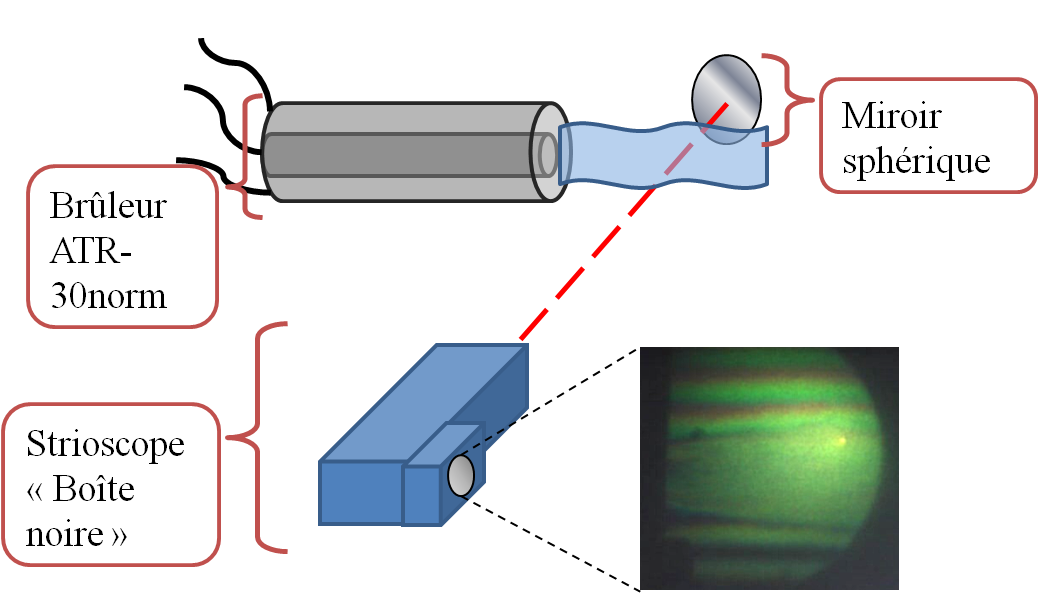
\includegraphics[width=0.6\textwidth]{fig/Schema_strio.png}
  \caption{The strioscopy experiment}
 \label{schema_strio}
\end{figure}
\subsubsection{The diagnostic of strioscopy }

There many kinds of strioscopy, the global aim is to measure the difference of optical path between two coherent beams. A difference of optical path induce a difference of density according to Gladstone-Dale law : $n-1=\kappa  \rho$. 

The strioscopy available at CRCD is interferential strioscopy, whose principle is described here :
\begin{figure}[!h]
  \centering
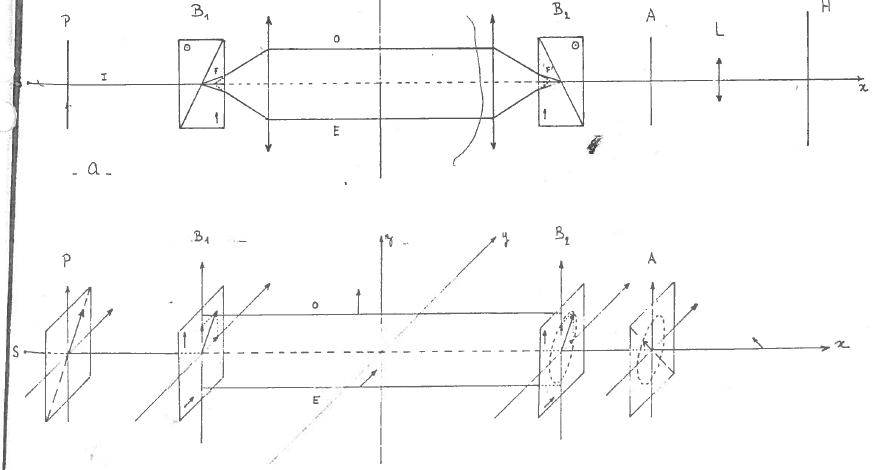
\includegraphics[width=0.8\textwidth]{fig/Principe_Strio.PNG}
  \caption{The strioscopy diagnostic}
 \label{principe_strio}
\end{figure}
A mercury source light (S) polarized by a polarizer (P) is divided into two coherent beams with a 1st biprism (B1). If the optical path between the two beams are equal, the 2nd biprism (B2) will gather the two beams, so that the polarization plan will be the same as before. A second polarizer works as an analyzer (A) : it  has a polarization plan perpendicular to the 1st polariszer, so that if the beam is not modified, no beam will be transmitted through the analyzer.

In case of a difference of optical path in the volume we want to measure, the polarization plan of the beam leaving the second biprism (B2) will not be the same, and its projection on the perpendicular polarization plan of the analyzer (A) will not be equal to zero anymore.

A fringe set up can be obtained by translating the second biprism along x-axis : without any perturbation of the measurement volume, the difference of optical path is then going to depend on the coordinate of the beam, so that parallel interferential fringes will appear in the absence of  perturbation of the measurement volume. The fringe set-up is responsible for the observation on figure \ref{image_strio} : when there is no pertubation, the fringes are strictly parallel, we can here observe a boundary layer at the proximity of the solid body thanks to the disposal.

\begin{figure}[!h]
  \centering
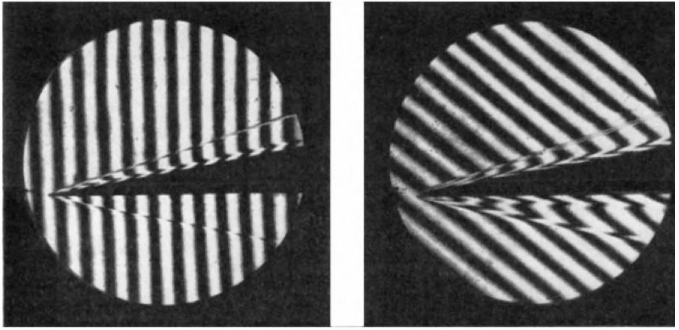
\includegraphics[width=0.8\textwidth]{fig/Strioscopie.PNG}
  \caption{The strioscopy diagnostic}
 \label{image_strio}
\end{figure}


\subsubsection{Procedure}

\begin{enumerate}
\item On a table, install the strioscope device
\item install the spherical mirror 3 meters ahead the lens of the strioscope
\item To calibrate the device, you can : \begin{itemize}
\item control the translation of the optical device (particularly, two configurations can be reached (by moving the strioscope along the optical axe): flat-colour or with fringe, in the case of fringes, one can change the position of the fringes by moving the biprism laterally)
\item choose the angle of the biprism ($1^\circ$,$2^\circ $ or $3^\circ$)
\item control the movement of the refringent bi-prism
\item In order to make the focus : control the drum with 8 positions for lenses, and then adjust it manually with the secondary fine controlling button (at the end of that point, the focus is supposed to be done on the examined object)
\item Change the device on which the final image is reflected (it can be a dulled glass, or a photographic plate, or a camera fixed to a support, or a screen)
\end{itemize}
\item One can check the set up with a small flame from a lighter
\end{enumerate}
\subsubsection{To take into account}
\paragraph{Protect the flow from the wind} It is absolutely necessary not to be under the influence of the wind. The best option is to make it indoor.

\paragraph{Taking care with the outlet temperature} Y. Joumani had troubles with keeping the outlet temperature because of the cooling inside the pipe. We have to measure it at the outlet (with thermocouple, for every used mass flow!) but also to insulate the pipes, or preheat a lot the initial gaz.

\paragraph{To test if the burner is really axisymetrical} Turn the burner and compare the results

\subsubsection{To include in the planning}
\begin{itemize}
\item CCD camera
\item Preheater
\end{itemize}
\section{The sizing of the reheater for the strioscopy}

  This is a compromise between the need for the experiment and the difficulty to craft the facility. This is a problem of heat transfer : with a given mass flow $\dot{m}=20.5 kg/h$, we want to heat air from ambient temperature to $T_{outlet}=605^\circ C$ with a hoven of maximal temperature $T_{hoven}=850^\circ C$. A simple OD model gives the energy balance :
  
  $\dot{m} c_{p} (T_{outlet} -T_{inlet})=(T_{hoven}-T_{mixture}) h S_{wet}$
  
  We use the correlation heat transfer : 
  
  $h=0.023 Re^{4/5} Pr^{0.3}$,  we introduce the length :$x_{0}=\frac{c_{p} \dot{m}^{1/5}D^{4/5}}{\lambda Pr^{0.3} 0.023 (4/(\mu \pi)^{4/5}\pi}$ 
 
and we find with a 0D model the necessary length $L$ to reach the outlet temperature : $L=x_{0} \frac{T_{outlet} -T_{inlet}}{T_{hoven}-T_{mixture}}$ 

and with a 1D model : $L=-x_{0} ln(1-\frac{T_{outlet} -T_{inlet}}{T_{hoven}-T_{inlet}})$  

The figure \ref{heater_sizing} shows that the two models are quite close at 1st order, we have to choose a technical solution with a reliable velocity (less than 30). Margins has been taken in this scenario, knowing that the pipe will not be at the exact temperature of the hoven, and that we want to over heat the flow at the outlet to compensate the thermal loss to reach the burner.

\begin{figure}[!h]
  \centering
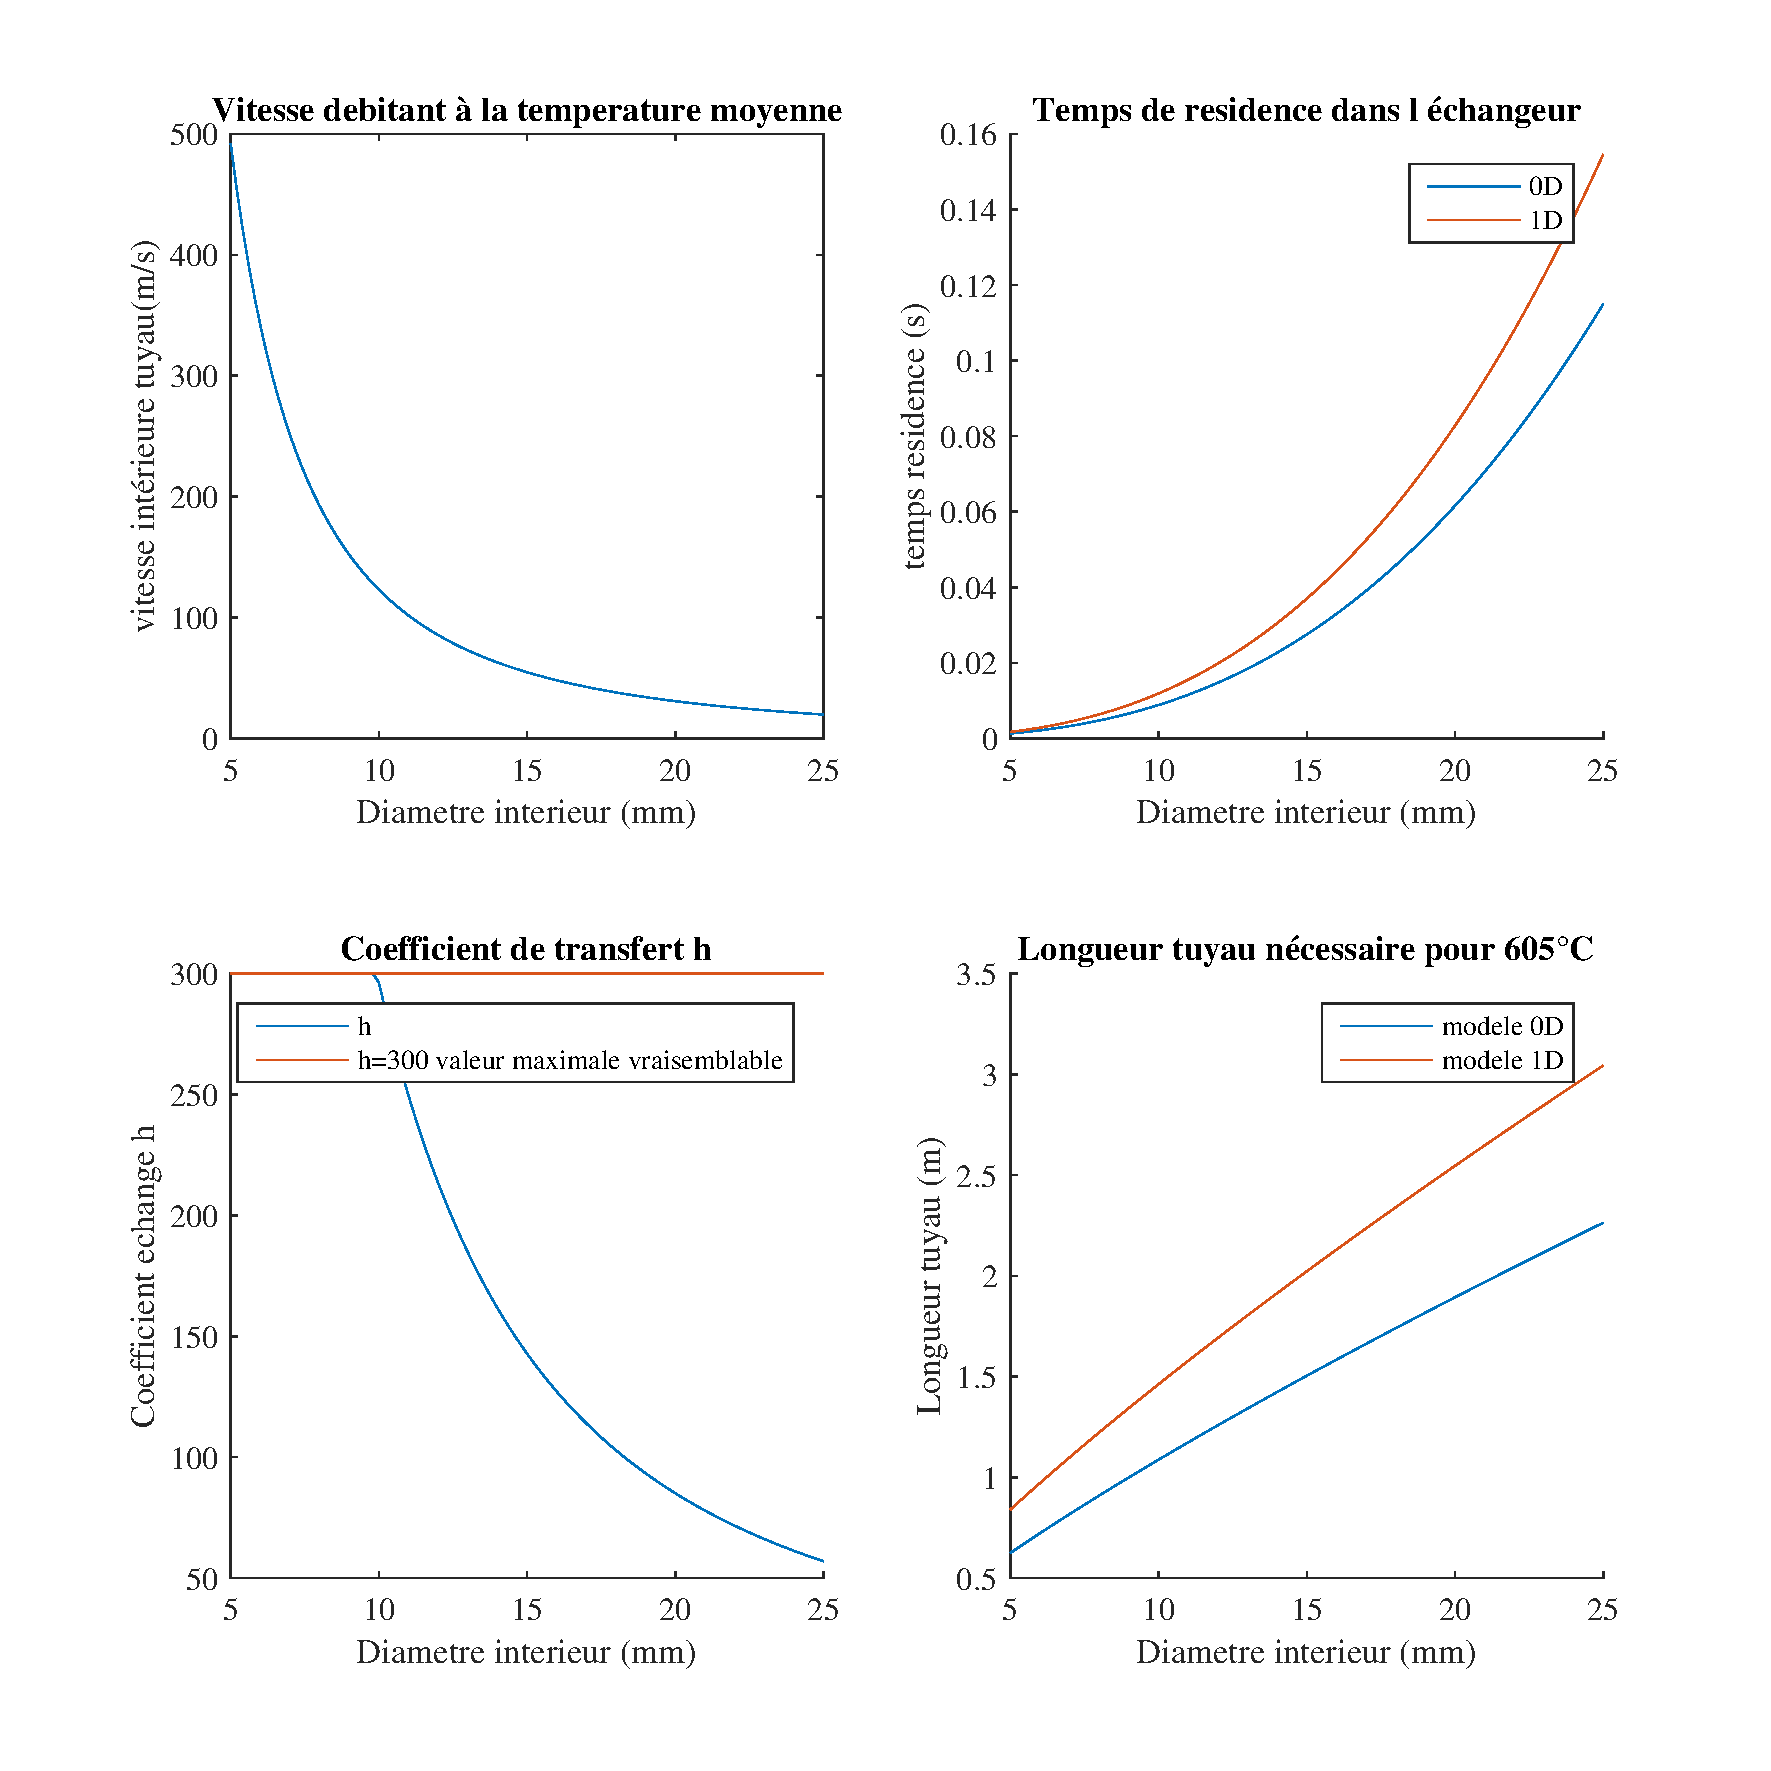
\includegraphics[width=0.9\textwidth]{fig/dimensionnement_rechauffeur.pdf}
  \caption{The heater sizing}
 \label{heater_sizing}
\end{figure}

Depending on what can be crafted, we may choose a 6meters long pipe of 20mm as internal diameter.